\documentclass[tikz]{standalone}

\usepackage{tikz}
\usepackage{pgfplots}
\pgfplotsset{compat=1.9}

\usetikzlibrary{math}
\usetikzlibrary{arrows.meta}


\begin{document}
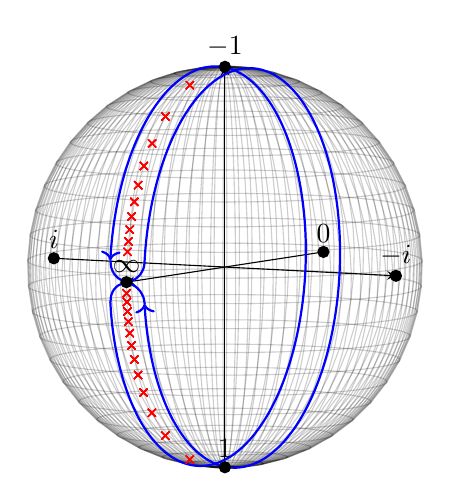
\begin{tikzpicture}
    \tikzmath{
        \r = 0.1;   % radius of curve to inf
        \t = 6;     % how far the curve is rotaed
    }
    \begin{axis}[axis lines=center, ticks=none, view/h=120, view/v=5]
    % Sphere
    \addplot3[%
    opacity = 0.1,
    mesh,
    black,
    z buffer = sort,
    samples = 50,
    variable = \u,
    variable y = \v,
    domain = 0:180,
    y domain = 0:360,
    ]
    ({cos(u)*sin(v)}, {sin(u)*sin(v)}, {cos(v)});
    % Large circles
    \addplot3[%
        domain=rad(\t):2*pi-rad(\t),
        samples=100,
        samples y=0,
        no marks,
        smooth,
        thick,
        blue,
        ->
    ]
    (
        {sqrt(1 - \r^2)*cos(deg(x))}, 
        {\r}, 
        {sqrt(1 - \r^2)*sin(deg(x))}
    );
    %
    \addplot3[%
        domain=rad(\t):2*pi-rad(\t),
        samples=100,
        samples y=0,
        no marks,
        smooth,
        thick,
        blue,
        <-
    ]
    (
        {sqrt(1 - \r^2)*cos(deg(x))}, 
        {-\r},
        {sqrt(1 - \r^2)*sin(deg(x))}
    );
    % Small curves touching infinity
    \addplot3[%
        domain=pi:2*pi,
        samples=10,
        samples y=0,
        no marks,
        smooth,
        thick,
        blue
    ]
    (   {1*cos(\t) - \r*sin(deg(x))*sin(\t)},
        {\r*cos(deg(x))+0.004},
        {1*sin(\t) + \r*sin(deg(x))*cos(\t)}
    );
    %
    \addplot3[%
        domain=0:pi,
        samples=10,
        samples y=0,
        no marks,
        smooth,
        thick,
        blue
    ]
    (   {1*cos(-\t) - \r*sin(deg(x))*sin(-\t)},
        {\r*cos(deg(x))+0.004},
        {1*sin(-\t) + \r*sin(deg(x))*cos(-\t)}
    );
    % Points
    \addplot3[
        mark=*,
        black, 
        point meta=explicit symbolic,
        nodes near coords
        ]
    coordinates {(1,0,0)[$\infty$]};
    \addplot3[
        mark=*,
        black, 
        point meta=explicit symbolic,
        nodes near coords
        ]
    coordinates {(-1,0,0)[$0$]};
    \addplot3[
        mark=*,
        black, 
        point meta=explicit symbolic,
        nodes near coords
        ]
    coordinates {(0,0,1)[$-1$]};
    \addplot3[
        mark=*,
        black, 
        point meta=explicit symbolic,
        nodes near coords
        ]
    coordinates {(0,0,-1)[$1$]};
    \addplot3[
        mark=*,
        black, 
        point meta=explicit symbolic,
        nodes near coords
        ]
    coordinates {(0,1,0)[$-i$]};
    \addplot3[
        mark=*,
        black, 
        point meta=explicit symbolic,
        nodes near coords
        ]
    coordinates {(0,-1,0)[$i$]};
    \addplot3[
        domain=2:15,
        samples=10,
        red,
        only marks,
        mark=x,
        ]
    (
        {cos(deg( pi/2* (ln(20) - ln(x))/ln(20)) )},
        {0},
        {sin(deg( pi/2* (ln(20) - ln(x))/ln(20)) ))}
    );
    \addplot3[
        domain=2:18,
        samples=12,
        red,
        only marks,
        mark=x,
        ]
    (
        {cos(deg( -pi/2* (ln(20) - ln(x))/ln(20)) )},
        {0},
        {sin(deg( -pi/2* (ln(20) - ln(x))/ln(20)) ))}
    );
    \end{axis}
\end{tikzpicture}
\end{document}
